\documentclass[11pt,a4paper]{article}
\usepackage[T1]{fontenc}
\usepackage[utf8]{inputenc}
\usepackage{lmodern}
\usepackage[margin=22mm,headheight=16pt]{geometry}
\usepackage{amsmath,amssymb,graphicx,array,longtable,booktabs}
\usepackage{microtype,xcolor,hyperref,xurl,fancyhdr}
\definecolor{Navy}{HTML}{17324D}
\definecolor{Teal}{HTML}{087F8C}
\definecolor{Gold}{HTML}{B88128}
\hypersetup{colorlinks=true,linkcolor=Navy,urlcolor=Teal,bookmarksnumbered=true,hypertexnames=false}
\setlength{\parindent}{0pt}
\setlength{\parskip}{6pt}
\setlength{\emergencystretch}{4em}
\setcounter{tocdepth}{1}
\pagestyle{fancy}\fancyhf{}
\fancyfoot[R]{\small\thepage}
\fancyfoot[L]{\small\sffamily Sharif University of Technology}
\renewcommand{\headrulewidth}{0.3pt}
\makeatletter
\renewcommand\section{\@startsection{section}{1}{\z@}{-3.2ex plus -1ex minus -.2ex}{1.6ex plus .2ex}{\normalfont\Large\sffamily\bfseries\color{Navy}}}
\renewcommand\subsection{\@startsection{subsection}{2}{\z@}{-2.5ex plus -1ex minus -.2ex}{1.2ex plus .2ex}{\normalfont\large\sffamily\bfseries\color{Teal}}}
\makeatother
\fancyhead[L]{\small\sffamily Reza Sanaee Nezhad}\fancyhead[R]{\small\sffamily Technical Report}\begin{document}
\begin{titlepage}\centering\vspace*{7mm}

\includegraphics[width=31mm]{assets/sharif_emblem_en.png}\par\vspace{5mm}
{\Large\sffamily\bfseries\color{Navy}SHARIF UNIVERSITY OF TECHNOLOGY\par}
\vspace{3mm}{\sffamily Department of Electrical Engineering\par}
\vspace{18mm}{\color{Teal}\rule{\linewidth}{1.4pt}}\par\vspace{6mm}
{\large\sffamily\color{Teal}TECHNICAL REPORT\par}
\vspace{9mm}{\huge\sffamily\bfseries\color{Navy}Cache-Aware SIMD and Strassen Matrix Multiplication\par}
\vspace{10mm}{\color{Gold}\rule{45mm}{1pt}}\par\vfill
\begin{minipage}{.88\linewidth}{\sffamily\color{Teal}AUTHOR}\par{\Large\sffamily Reza Sanaee Nezhad}\par Student ID: 401101502\par\vspace{9mm}
{\sffamily\color{Teal}INSTRUCTOR}\par
Not identified in the supplied materials\par
\end{minipage}\vfill\end{titlepage}
\tableofcontents\clearpage
\section{Objective and computational problem}

This project computes the product of two square matrices of double-precision values and compares a direct reference implementation with a hybrid implementation that combines memory-layout transformation, a four-by-four SIMD microkernel, and Strassen recursion. The mathematical contract is C[i,j] =\allowbreak{} sum over k of A[i,k] times B[k,j], for i,j,k from zero to n-1. The inputs are read-only and the output occupies separate storage. Each matrix is row-major, and an explicit leading dimension specifies the distance between successive rows. A logical n-by-n submatrix can therefore be processed within a larger parent allocation without copying its rows into a separate matrix.


The direct path preserves the simple pointer-based multiplication used as a numerical reference. The optimized path first makes the inner products contiguous, then evaluates multiple output elements together. Strassen reduces the number of recursive products from eight to seven when a matrix is split into four equal quadrants. The crossover between arithmetic savings and preparation overhead is controlled by a leaf threshold. The default threshold is 512, matching the intended hybrid structure. Dimensions at or below that threshold use the transposed leaf kernel directly. Odd dimensions also use that kernel because an equal-quadrant split is not defined for them.

\section{Row-major layout, strides, and the reference algorithm}

For a row-major matrix A with leading dimension s\_\allowbreak{}A, element A[i,k] is stored at offset i*s\_\allowbreak{}A+\allowbreak{}k. In the reference i-j-k loop, A's row is read sequentially, while B[k,j] advances by s\_\allowbreak{}B doubles at each inner-loop iteration. C[i,j] is written only after its dot product has been accumulated. The algorithm performs n cubed scalar multiplications and approximately n cubed additions. Its arithmetic complexity is cubic even when pointer arithmetic replaces repeated array indexing.


The strided traversal of B can reduce spatial locality:\allowbreak{} consecutive values used by one dot product may reside in different cache lines, and a large working set can repeatedly displace useful data. The source-level use of register variables does not guarantee a particular hardware-register allocation. The compiler determines that allocation. This project consequently identifies the memory access pattern and arithmetic scheduling explicitly instead of treating a language keyword as a measured optimization.


The public reference function accepts separate s\_\allowbreak{}A, s\_\allowbreak{}B and s\_\allowbreak{}C values. This matters for the validation experiments, which deliberately use different padded row lengths. A correct result must be stored only in the first n entries of each output row;\allowbreak{} the padding after those entries is left intact. The same contract applies to the recursive and SIMD paths.

\section{Transposing the second operand}

The leaf routine allocates a packed n-by-n buffer B\_\allowbreak{}T and stores B\_\allowbreak{}T[j*n+\allowbreak{}k] =\allowbreak{} B[k*s\_\allowbreak{}B+\allowbreak{}j]. An inner product then reads both A[i*s\_\allowbreak{}A+\allowbreak{}k] and B\_\allowbreak{}T[j*n+\allowbreak{}k] sequentially. Transposition requires quadratic preparation work and an additional n squared doubles. The buffer is released after the leaf product, including the scalar fallback path.


The allocation has 64-byte alignment. Row starts and submatrix offsets are not assumed to retain that alignment. Unaligned AVX loads and stores are therefore used for vector operations, which makes the kernel valid for padded strides and submatrix views. Alignment of the allocation and alignment of every accessed vector are separate properties.


The timing of the optimized function includes this transpose, its allocation and deallocation, arithmetic, and any recursive temporary storage. It is an end-to-end multiplication time rather than a measurement of arithmetic instructions alone. For small matrices the preparation cost can consume much of the arithmetic benefit. No hardware cache-miss counters are collected, so locality is explained from the access pattern and not presented as a measured cache-miss reduction.

\section{Four-by-four AVX leaf microkernel}

An output tile contains up to four rows and four columns. For each group of four k values, the kernel loads one four-double vector from each participating A row and one from each participating B\_\allowbreak{}T row. Every A vector is reused against the B\_\allowbreak{}T vectors for that tile, and every B\_\allowbreak{}T vector is reused against the A vectors. Sixteen independent vector accumulators represent a complete four-by-four tile. The operations are vector multiplication followed by vector addition;\allowbreak{} fused multiply-add is not required.


After the vector loop, each accumulator's four lanes are summed to produce one output scalar. Remaining k values are accumulated scalarly. Partial tiles at the last rows or columns are also handled explicitly. Thus n need not be divisible by four. A one-by-one matrix, a three-by-three matrix and a matrix with an odd leading dimension obey the same indexing contract as a large matrix.


The AVX routine is isolated in a target-specific function when compiled with GCC on x86. Runtime CPU dispatch selects it only when AVX is available. Otherwise the routine uses the same transposed storage with scalar dot products. Defining MATRIX\_\allowbreak{}DISABLE\_\allowbreak{}AVX builds the scalar path alone. The reference, allocation, recursion, comparison and command-line code do not require a global -mavx compiler flag. The distributed test suite exercises both the AVX-capable build and the scalar-only build.

\section{Strassen partitioning and seven recursive products}

For an even dimension n above the leaf threshold, m=\allowbreak{}n/\allowbreak{}2. A and B are partitioned into A11, A12, A21, A22 and B11, B12, B21, B22. Each quadrant is a view into its parent allocation, with its parent's leading dimension. The seven products follow the standard Strassen identities shown below. Temporary sums and differences are packed m-by-m matrices. The output products M1 through M7 are also packed, while the final C quadrants use the caller's output stride.


The products are evaluated sequentially. Two temporary matrices hold sums and differences, and their contents are reused once the corresponding recursive multiplication has completed. Seven product matrices retain the intermediate results needed for final recombination. Additions and subtractions use both source strides explicitly, so a parent view and a packed temporary need not share a row length.


Every recursive call receives its logical dimension and all three leading dimensions separately. The logical dimension is not inferred from an output stride. A nonzero cutoff is required. Even dimensions greater than the cutoff are split recursively;\allowbreak{} a small or odd subproblem is computed by the complete leaf kernel. This avoids discarding an unmatched last row or column. It also means that the familiar Strassen asymptotic bound applies to the repeatedly splittable case, while an odd problem may use cubic leaf work.

\begin{align*}
M_1&=(A_{11}+A_{22})(B_{11}+B_{22}), & M_2&=(A_{21}+A_{22})B_{11},\\
M_3&=A_{11}(B_{12}-B_{22}), & M_4&=A_{22}(B_{21}-B_{11}),\\
M_5&=(A_{11}+A_{12})B_{22}, & M_6&=(A_{21}-A_{11})(B_{11}+B_{12}),\\
M_7&=(A_{12}-A_{22})(B_{21}+B_{22}).
\end{align*}\clearpage
\section{Recombination, storage, and complexity}

The output quadrants are obtained from the seven products using the recombination equations below. Each element is written at the correct offset in the caller's C allocation. The implementation does not overwrite A or B. The input and output buffers must not overlap because the computation reads input values throughout the multiplication.


For repeated even splits, the recurrence is T(n)=\allowbreak{}7*T(n/\allowbreak{}2)+\allowbreak{}O(n squared), which gives O(n to the power log2(7)), approximately O(n to the power 2.8074), rather than cubic arithmetic. This is an arithmetic-count statement, not a guarantee of lower elapsed time for every n. Transposition, matrix addition, allocation and memory traffic influence the crossover in practice.


Nine m-by-m temporary arrays are held at one recursive level:\allowbreak{} seven products and two work matrices. A descending sequential call adds further temporary levels, and its leaf adds one transpose buffer. For n=\allowbreak{}1024 with cutoff 512, the top-level temporaries occupy 18 MiB and a 512-by-512 transpose occupies 2 MiB. The four main 1024-by-1024 double arrays occupy 32 MiB, giving approximately 52 MiB of matrix storage at the peak, excluding allocator and runtime overhead. No measured resident-memory trace is claimed.


An allocation failure propagates to the caller. Allocations already obtained by that call are released before returning failure. Matrix dimensions and leading dimensions are checked before entering the kernel. Allocation-size calculations use size\_\allowbreak{}t and guard multiplication overflow. The benchmark accepts positive dimensions and cutoffs up to 8192 and reports allocation failure instead of continuing with a null pointer.

\begin{align*}
C_{11}&=M_1+M_4-M_5+M_7, & C_{12}&=M_3+M_5,\\
C_{21}&=M_2+M_4, & C_{22}&=M_1-M_2+M_3+M_6.
\end{align*}\clearpage
\section{Floating-point agreement and numerical validation}

Floating-point products can differ because SIMD lane reduction and Strassen recombination change the order of arithmetic. Exact bitwise equality is therefore not the numerical contract. Each result element must satisfy an absolute-plus-relative error bound:\allowbreak{} absolute error no greater than atol +\allowbreak{} rtol*max(abs(reference),abs(candidate)). Nonfinite values cause comparison failure. The rule remains defined when the reference value is zero, unlike division by the reference value.


The deterministic test suite uses dimensions 1,2,3,4,5,7,8,12,16,31,32,33 and 64. Each dimension is tested with four patterns:\allowbreak{} a zero left operand, an identity left operand, an identity right operand, and signed nontrivial operands. A cutoff of four exercises multiple recursive levels. Leading dimensions n+\allowbreak{}3, n+\allowbreak{}5 and n+\allowbreak{}7 test independent row strides. Output padding is initialized with a sentinel and checked after every multiplication. This yields 52 matrix cases per backend. Both AVX-capable and scalar-only builds pass all 52 cases, as well as explicit zero and nonfinite comparison checks. The tests use atol=\allowbreak{}rtol=\allowbreak{}1e-10 for their bounded signed inputs.


The measured benchmark uses larger positive rational inputs and compares every element against the direct reference with atol=\allowbreak{}1e-8 and rtol=\allowbreak{}1e-10. All fifteen benchmark executions pass that criterion. The maximum absolute error is also recorded;\allowbreak{} its magnitude alone is not the pass criterion because the result values vary in scale.

\[|x-y|\leq\mathrm{atol}+\mathrm{rtol}\max(|x|,|y|).\]
\clearpage
\section{Benchmark procedure and measured results}

The benchmark is single-threaded. It was compiled with GCC at -O3 and run on Windows on an Intel Core i7-13650HX with AVX enabled. Inputs are generated deterministically from seed 42. The allocation and initialization of the four main matrices occur before timing;\allowbreak{} the optimized function's internal allocations and transposition occur inside its timed interval. Windows QueryPerformanceCounter provides elapsed wall-clock time. Each dimension is run three times, always with cutoff 512. The baseline is timed before the optimized path in each process.


The table reports the median reference time, median optimized time, minimum-to-maximum optimized time and median of the three per-run speedup ratios. The speedup column is not calculated by dividing the two separately chosen medians. The underlying CSV retains every repetition and its numerical check. Dimensions 64 through 512 use the AVX/\allowbreak{}transposed leaf directly;\allowbreak{} n=\allowbreak{}1024 uses one Strassen split into seven 512-dimensional leaf products.


These timings describe this machine and executable. The three repetitions are a descriptive sample, not a confidence interval or a general performance guarantee. The large spread at n=\allowbreak{}1024 and the first-run difference at n=\allowbreak{}256 show the influence of execution conditions. The comparison does not isolate the independent contribution of transposition, AVX tiling and Strassen, nor compare against a tuned BLAS library. Such ablations and additional machines would be needed for broader architectural conclusions.

\begingroup\small\setlength{\tabcolsep}{4pt}\renewcommand{\arraystretch}{1.22}\begin{longtable}{@{}llll@{}}
\caption{Three-repetition elapsed-time and speedup summary}\\\toprule
\textbf{n} & \textbf{Reference median (s)} & \textbf{Hybrid median (s)} & \textbf{Median speedup} \\ \midrule\endfirsthead \textbf{n} & \textbf{Reference median (s)} & \textbf{Hybrid median (s)} & \textbf{Median speedup} \\ \midrule\endhead
64 & 0.0000823 & 0.0000755 & 1.089x \\
128 & 0.0010332 & 0.0003716 & 2.782x \\
256 & 0.0083293 & 0.0021023 & 3.962x \\
512 & 0.2969118 & 0.0161739 & 18.326x \\
1024 & 2.5930254 & 0.1354898 & 18.578x \\
\bottomrule\end{longtable}\endgroup
\begingroup\small\setlength{\tabcolsep}{4pt}\renewcommand{\arraystretch}{1.22}\begin{longtable}{@{}llll@{}}
\caption{Timing variability and numerical errors; all repetitions verified}\\\toprule
\textbf{n} & \textbf{Hybrid minimum (s)} & \textbf{Hybrid maximum (s)} & \textbf{Maximum abs. error} \\ \midrule\endfirsthead \textbf{n} & \textbf{Hybrid minimum (s)} & \textbf{Hybrid maximum (s)} & \textbf{Maximum abs. error} \\ \midrule\endhead
64 & 0.0000619 & 0.0000759 & 4.6566e-10 \\
128 & 0.0003495 & 0.0003812 & 4.6566e-10 \\
256 & 0.0019818 & 0.0036748 & 1.4901e-08 \\
512 & 0.0148171 & 0.0163146 & 1.4901e-08 \\
1024 & 0.1103774 & 0.1902467 & 2.3842e-07 \\
\bottomrule\end{longtable}\endgroup
\begin{figure}[!htbp]\centering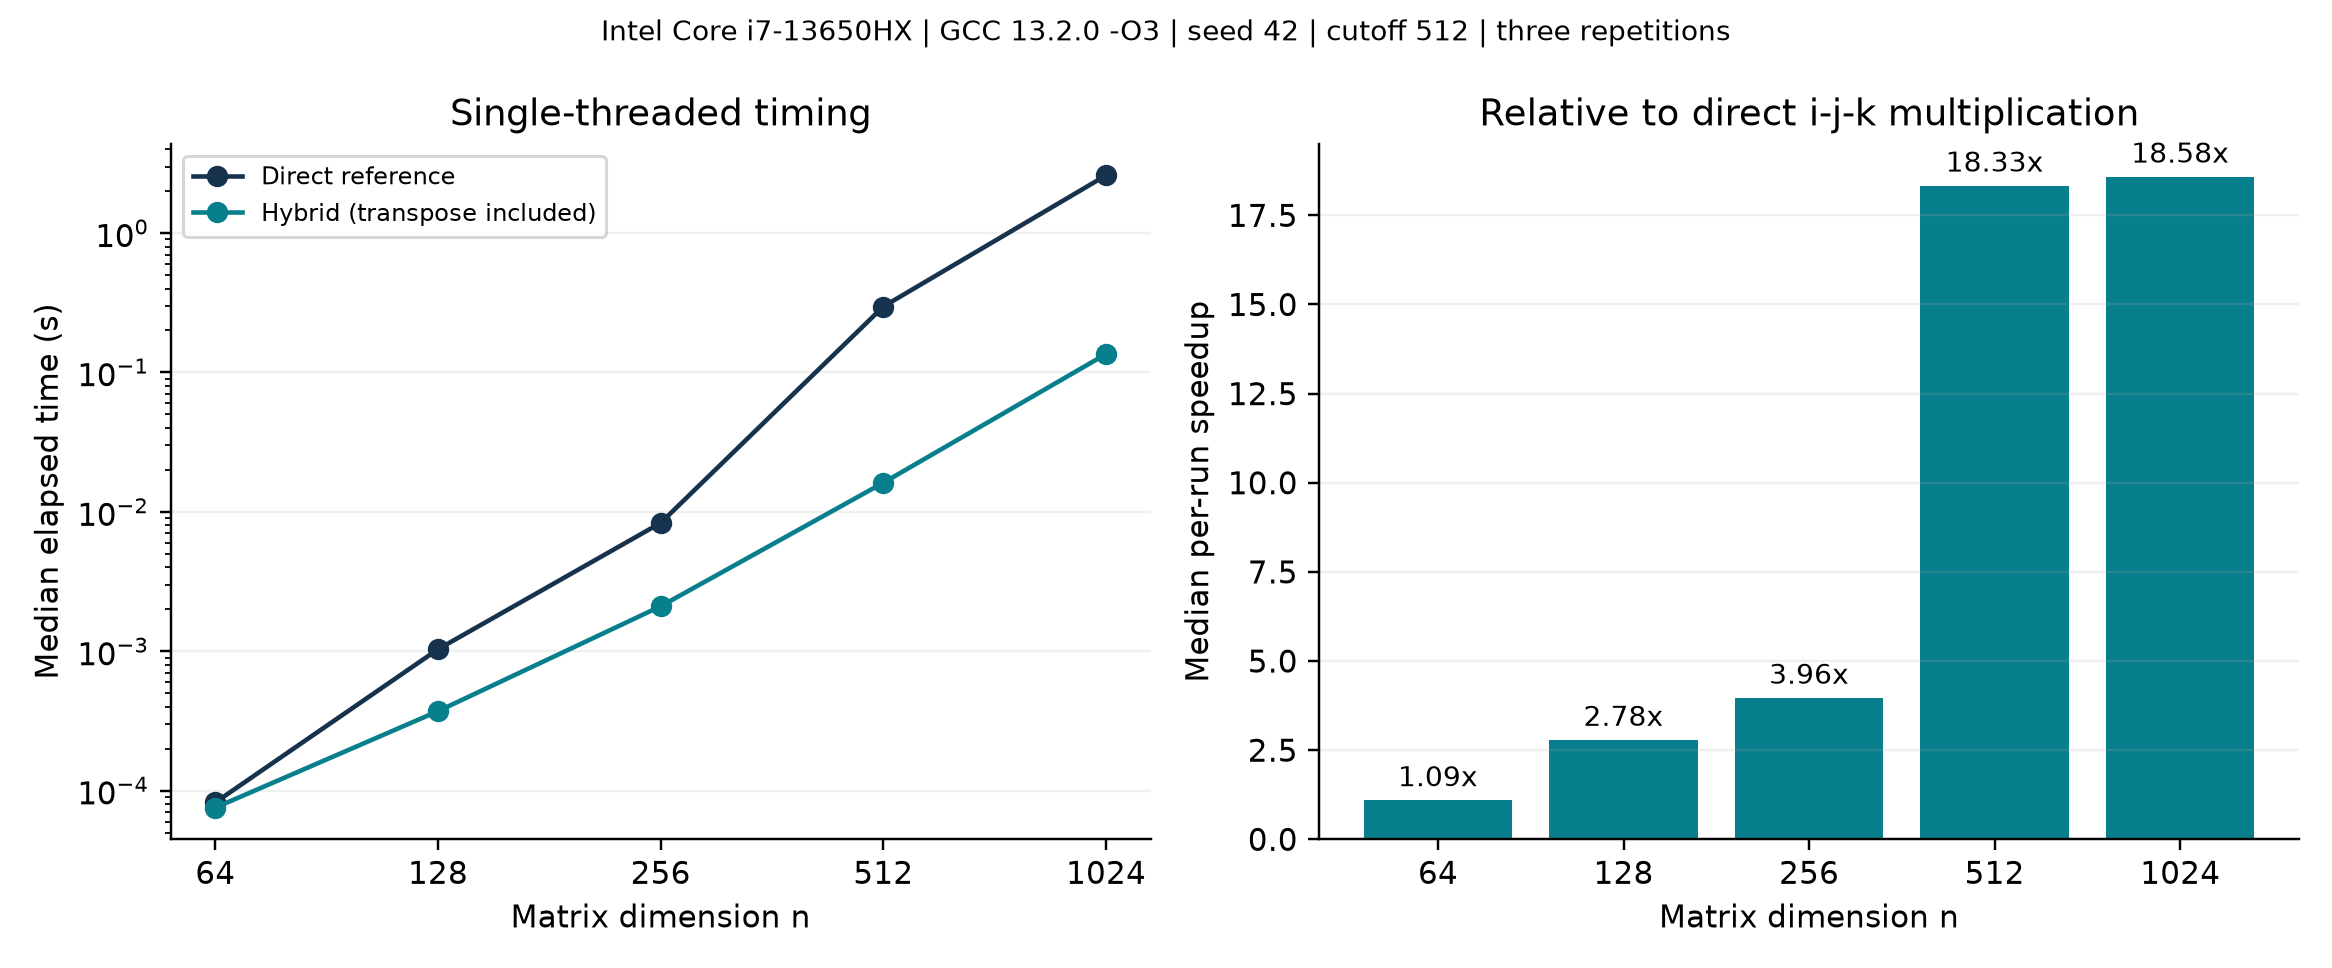
\includegraphics[width=\linewidth,height=.70\textheight,keepaspectratio]{assets/benchmark_results.png}\caption{Measured timing and median per-run speedup on the stated processor. Preparation internal to the hybrid product is included.}\end{figure}
\clearpage
\section{Build, execution, and interpretation}

The code package separates the matrix library, command-line benchmark, deterministic tests and measured CSV. On Windows, build.ps1 compiles the benchmark and tests with MinGW GCC and executes the tests. On a POSIX system, make and make test provide the corresponding build. The benchmark accepts dimension, leaf cutoff and seed as positional arguments. A run such as matrix\_\allowbreak{}benchmark 1024 512 42 emits a CSV header and one measurement row. Every measurement includes the AVX-dispatch state, both elapsed times, speedup, maximum absolute error and verification flag.


The resulting implementation demonstrates memory-layout transformation, tiled vector arithmetic, recursive matrix algorithms and numerical validation in one program. Its conclusions are limited to measured end-to-end timing and verified numerical agreement for the stated inputs. It does not measure power, prove a universal cache policy improvement or establish optimal performance across processors.

\clearpage\appendix\section{Implementation details}
\subsection{matrix.h}
\begin{figure}[!htbp]\begin{minipage}{\linewidth}\fontsize{10}{11.4}\selectfont\begin{verbatim}
#ifndef MATRIX_H
#define MATRIX_H
#include <stddef.h>
double *matrix_alloc(size_t rows, size_t stride);
void matrix_free(double *p);
void matrix_mult_ptr_reg(size_t n, const double *a, size_t sa,
                         const double *b, size_t sb, double *c, size_t sc);
int matrix_mult_base_stride(size_t n, const double *a, size_t sa,
                            const double *b, size_t sb, double *c, size_t 
    sc);
int strassen_stride(size_t n, const double *a, size_t sa, const double *b,
                    size_t sb, double *c, size_t sc, size_t cutoff);
int matrix_has_avx(void);
int matrix_compare(size_t n, const double *a, size_t sa, const double *b,
                    size_t sb, double atol, double rtol, double *max_error);
#endif
\end{verbatim}\end{minipage}\caption{Implementation: matrix.h.}\end{figure}
\clearpage
\subsection{matrix.c}
\begin{figure}[!htbp]\begin{minipage}{\linewidth}\fontsize{10}{11.4}\selectfont\begin{verbatim}
#define _POSIX_C_SOURCE 200112L
#include "matrix.h"
#include <stdlib.h>
#include <stdint.h>
#include <math.h>
#ifdef _WIN32
#include <malloc.h>
#endif
#if defined(__GNUC__) && (defined(__x86_64__) || defined(__i386__)) && 
    !defined(MATRIX_DISABLE_AVX)
#include <immintrin.h>
#define HAVE_AVX_KERNEL 1
#endif

double *matrix_alloc(size_t rows, size_t stride) {
    if (!rows || !stride || rows > SIZE_MAX / stride / sizeof(double)) 
    return NULL;
    size_t bytes = rows * stride * sizeof(double);
#ifdef _WIN32
    return (double *)_aligned_malloc(bytes, 64);
#else
    void *p = NULL;
    return posix_memalign(&p, 64, bytes) == 0 ? p : NULL;
#endif
}
void matrix_free(double *p) {
#ifdef _WIN32
    _aligned_free(p);
#else
    free(p);
#endif
}
int matrix_has_avx(void) {
#ifdef HAVE_AVX_KERNEL
    __builtin_cpu_init();
    return __builtin_cpu_supports("avx") != 0;
#else
    return 0;
#endif
}
void matrix_mult_ptr_reg(size_t n, const double *a, size_t sa,
                         const double *b, size_t sb, double *c, size_t sc) {
    for (size_t i = 0; i < n; ++i)
        for (size_t j = 0; j < n; ++j) {
            double sum = 0.0;
            for (size_t k = 0; k < n; ++k) sum += a[i*sa+k] * b[k*sb+j];
\end{verbatim}\end{minipage}\caption{Implementation: matrix.c (panel 1 of 4).}\end{figure}
\begin{figure}[!htbp]\begin{minipage}{\linewidth}\fontsize{10}{11.4}\selectfont\begin{verbatim}
            c[i*sc+j] = sum;
        }
}
#ifdef HAVE_AVX_KERNEL
__attribute__((target("avx")))
static void leaf_avx(size_t n, const double *a, size_t sa,
                      const double *bt, double *c, size_t sc) {
    /* Sixteen vector accumulators evaluate a 4 x 4 output tile. */
    for (size_t i = 0; i < n; i += 4)
        for (size_t j = 0; j < n; j += 4) {
            size_t nr = n-i < 4 ? n-i : 4, nc = n-j < 4 ? n-j : 4;
            __m256d acc[4][4];
            for (size_t r=0;r<nr;++r)
                for(size_t q=0;q<nc;++q) acc[r][q]=_mm256_setzero_pd();
            size_t k=0;
            for (; k+4<=n; k+=4) {
                __m256d av[4], bv[4];
                for(size_t r=0;r<nr;++r) 
    av[r]=_mm256_loadu_pd(a+(i+r)*sa+k);
                for(size_t q=0;q<nc;++q) 
    bv[q]=_mm256_loadu_pd(bt+(j+q)*n+k);
                for(size_t r=0;r<nr;++r)
                    for(size_t q=0;q<nc;++q)
                        
    acc[r][q]=_mm256_add_pd(acc[r][q],_mm256_mul_pd(av[r],bv[q]));
            }
            for(size_t r=0;r<nr;++r)
                for(size_t q=0;q<nc;++q) {
                    double lanes[4]; _mm256_storeu_pd(lanes,acc[r][q]);
                    double sum=lanes[0]+lanes[1]+lanes[2]+lanes[3];
                    for(size_t tail=k;tail<n;++tail) 
    sum+=a[(i+r)*sa+tail]*bt[(j+q)*n+tail];
                    c[(i+r)*sc+j+q]=sum;
                }
        }
}
#endif
int matrix_mult_base_stride(size_t n, const double *a, size_t sa,
                            const double *b, size_t sb, double *c, size_t 
    sc) {
    if(!n || sa<n || sb<n || sc<n) return 0;
    double *bt=matrix_alloc(n,n);if(!bt) return 0;
    for(size_t i=0;i<n;++i)
        for(size_t j=0;j<n;++j) bt[j*n+i]=b[i*sb+j];
#ifdef HAVE_AVX_KERNEL
    if(matrix_has_avx()) leaf_avx(n,a,sa,bt,c,sc);
\end{verbatim}\end{minipage}\caption{Implementation: matrix.c (panel 2 of 4).}\end{figure}
\begin{figure}[!htbp]\begin{minipage}{\linewidth}\fontsize{10}{11.4}\selectfont\begin{verbatim}
    else
#endif
    for(size_t i=0;i<n;++i)
        for(size_t j=0;j<n;++j) {
            double sum=0.0;
            for(size_t k=0;k<n;++k) sum+=a[i*sa+k]*bt[j*n+k];
            c[i*sc+j]=sum;
        }
    matrix_free(bt);return 1;
}
static void combine(size_t n,const double *a,size_t sa,const double 
    *b,size_t sb,
                      double *c,int subtract) {
    for(size_t i=0;i<n;++i)
        for(size_t j=0;j<n;++j) c[i*n+j]=a[i*sa+j]+(subtract ? -b[i*sb+j] : 
    b[i*sb+j]);
}
int strassen_stride(size_t n,const double *a,size_t sa,const double 
    *b,size_t sb,
                    double *c,size_t sc,size_t cutoff) {
    if(!n || sa<n || sb<n || sc<n || !cutoff) return 0;
    if(n<=cutoff || n%2) return matrix_mult_base_stride(n,a,sa,b,sb,c,sc);
    size_t m=n/2;double *p[9]={0};int ok=0;
    for(size_t i=0;i<9;++i) if(!(p[i]=matrix_alloc(m,m))) goto cleanup;
    const double *a11=a,*a12=a+m,*a21=a+m*sa,*a22=a+m*sa+m;
    const double *b11=b,*b12=b+m,*b21=b+m*sb,*b22=b+m*sb+m;
    double *t1=p[7],*t2=p[8];
#define PRODUCT(index,x,sx,y,sy) do { 
    if(!strassen_stride(m,x,sx,y,sy,p[index],m,cutoff)) goto cleanup; } 
    while(0)
    combine(m,a11,sa,a22,sa,t1,0);combine(m,b11,sb,b22,sb,t2,0);PRODUCT(0,t1
    ,m,t2,m);
    combine(m,a21,sa,a22,sa,t1,0);PRODUCT(1,t1,m,b11,sb);
    combine(m,b12,sb,b22,sb,t1,1);PRODUCT(2,a11,sa,t1,m);
    combine(m,b21,sb,b11,sb,t1,1);PRODUCT(3,a22,sa,t1,m);
    combine(m,a11,sa,a12,sa,t1,0);PRODUCT(4,t1,m,b22,sb);
    combine(m,a21,sa,a11,sa,t1,1);combine(m,b11,sb,b12,sb,t2,0);PRODUCT(5,t1
    ,m,t2,m);
    combine(m,a12,sa,a22,sa,t1,1);combine(m,b21,sb,b22,sb,t2,0);PRODUCT(6,t1
    ,m,t2,m);
#undef PRODUCT
    for(size_t i=0;i<m;++i)
        for(size_t j=0;j<m;++j) {
            size_t k=i*m+j,idx=i*sc+j;
            c[idx]=p[0][k]+p[3][k]-p[4][k]+p[6][k];
            c[idx+m]=p[2][k]+p[4][k];
\end{verbatim}\end{minipage}\caption{Implementation: matrix.c (panel 3 of 4).}\end{figure}
\begin{figure}[!htbp]\begin{minipage}{\linewidth}\fontsize{10}{11.4}\selectfont\begin{verbatim}
            c[idx+m*sc]=p[1][k]+p[3][k];
            c[idx+m*sc+m]=p[0][k]-p[1][k]+p[2][k]+p[5][k];
        }
    ok=1;
cleanup:
    for(size_t i=0;i<9;++i) matrix_free(p[i]);
    return ok;
}
int matrix_compare(size_t n,const double *a,size_t sa,const double *b,size_t
     sb,
                    double atol,double rtol,double *max_error) {
    int ok=1;*max_error=0.0;
    for(size_t i=0;i<n;++i)
        for(size_t j=0;j<n;++j) {
            double x=a[i*sa+j],y=b[i*sb+j],error=fabs(x-y);
            if(!isfinite(x)||!isfinite(y)) {ok=0;*max_error=INFINITY;}
            else {
                if(error>*max_error)*max_error=error;
                if(error>atol+rtol*fmax(fabs(x),fabs(y)))ok=0;
            }
        }
    return ok;
}
\end{verbatim}\end{minipage}\caption{Implementation: matrix.c (panel 4 of 4).}\end{figure}
\clearpage
\subsection{main.c}
\begin{figure}[!htbp]\begin{minipage}{\linewidth}\fontsize{10}{11.4}\selectfont\begin{verbatim}
#define _POSIX_C_SOURCE 200809L
#include "matrix.h"
#include <stdio.h>
#include <stdlib.h>
#include <stdint.h>
#include <errno.h>
#ifdef _WIN32
#include <windows.h>
#else
#include <time.h>
#endif
static double seconds(void) {
#ifdef _WIN32
    LARGE_INTEGER 
    t,f;QueryPerformanceCounter(&t);QueryPerformanceFrequency(&f);
    return (double)t.QuadPart/(double)f.QuadPart;
#else
    struct timespec t;clock_gettime(CLOCK_MONOTONIC,&t);return 
    t.tv_sec+t.tv_nsec*1e-9;
#endif
}
static uint32_t next_random(uint32_t *s) 
    {*s^=*s<<13;*s^=*s>>17;*s^=*s<<5;return *s;}
static int parse(const char *s,size_t *value) {
    if(!*s || *s=='-')return 0;
    char *end;errno=0;unsigned long long n=strtoull(s,&end,10);
    if(errno || *end || n<1 || n>8192)return 0;
    *value=(size_t)n;return 1;
}
int main(int argc,char **argv) {
    size_t n=128,cutoff=512,seed=42;
    if(argc>4 || (argc>1&&!parse(argv[1],&n)) || 
    (argc>2&&!parse(argv[2],&cutoff)) || (argc>3&&!parse(argv[3],&seed))) {
        fprintf(stderr,"Usage: matrix_benchmark [dimension 1..8192] [cutoff 
    1..8192] [seed 1..8192]\n");return 2;
    }
    double *a=matrix_alloc(n,n),*b=matrix_alloc(n,n),*ref=matrix_alloc(n,n),
    *opt=matrix_alloc(n,n);
    if(!a||!b||!ref||!opt){fprintf(stderr,"Memory allocation failed\n");matr
    ix_free(a);matrix_free(b);matrix_free(ref);matrix_free(opt);return 2;}
    uint32_t state=(uint32_t)seed;
    for(size_t i=0;i<n*n;++i) {
        
    a[i]=(double)(1+next_random(&state)%12345)/(1+next_random(&state)%6789);
        
    b[i]=(double)(1+next_random(&state)%12345)/(1+next_random(&state)%6789);
\end{verbatim}\end{minipage}\caption{Implementation: main.c (panel 1 of 2).}\end{figure}
\begin{figure}[!htbp]\begin{minipage}{\linewidth}\fontsize{10}{11.4}\selectfont\begin{verbatim}
    }
    double t=seconds();matrix_mult_ptr_reg(n,a,n,b,n,ref,n);double 
    reference=seconds()-t;
    t=seconds();int allocated=strassen_stride(n,a,n,b,n,opt,n,cutoff);double
     optimized=seconds()-t;
    double error=0.0;int 
    pass=allocated&&matrix_compare(n,ref,n,opt,n,1e-8,1e-10,&error);
    puts("dimension,cutoff,seed,avx,reference_seconds,optimized_seconds,spee
    dup,max_absolute_error,verified");
    printf("%zu,%zu,%zu,%d,%.9f,%.9f,%.6f,%.12g,%d\n",n,cutoff,seed,matrix_h
    as_avx(),reference,optimized,optimized>0?reference/optimized:0,error,pas
    s);
    matrix_free(a);matrix_free(b);matrix_free(ref);matrix_free(opt);return 
    pass?0:1;
}
\end{verbatim}\end{minipage}\caption{Implementation: main.c (panel 2 of 2).}\end{figure}
\clearpage
\subsection{test\_matrix.c}
\begin{figure}[!htbp]\begin{minipage}{\linewidth}\fontsize{10}{11.4}\selectfont\begin{verbatim}
#include "matrix.h"
#include <stdio.h>
#include <stdlib.h>
#include <math.h>
#include <assert.h>
int main(void) {
    size_t sizes[]={1,2,3,4,5,7,8,12,16,31,32,33,64};size_t cases=0;
    for(size_t x=0;x<sizeof(sizes)/sizeof(sizes[0]);++x) {
        size_t n=sizes[x],sa=n+3,sb=n+5,sc=n+7;
        double *a=matrix_alloc(n,sa),*b=matrix_alloc(n,sb),*r=matrix_alloc(n
    ,sc),*o=matrix_alloc(n,sc);
        assert(a&&b&&r&&o);
        for(int kind=0;kind<4;++kind) {
            for(size_t i=0;i<n;++i)
                for(size_t j=0;j<n;++j) {
                    
    a[i*sa+j]=kind==0?0:kind==1?(i==j):((int)((i*13+j*7)%31)-15)/7.0;
                    b[i*sb+j]=kind==2?(i==j):((int)((i*5+j*11)%29)-14)/9.0;
                }
            for(size_t i=0;i<n*sc;++i)o[i]=1234567.0;
            matrix_mult_ptr_reg(n,a,sa,b,sb,r,sc);
            assert(strassen_stride(n,a,sa,b,sb,o,sc,4));
            double 
    error;assert(matrix_compare(n,r,sc,o,sc,1e-10,1e-10,&error));
            for(size_t i=0;i<n;++i)for(size_t 
    j=n;j<sc;++j)assert(o[i*sc+j]==1234567.0);
            ++cases;
        }
        matrix_free(a);matrix_free(b);matrix_free(r);matrix_free(o);
    }
    double z=0.0,nan=NAN,error;assert(!matrix_compare(1,&z,1,&nan,1,1e-
    10,1e-10,&error));
    assert(matrix_compare(1,&z,1,&z,1,1e-10,1e-10,&error));
    printf("PASS: %zu matrix cases; padded-stride guards; zero and nonfinite
     comparison; AVX=%d\n",cases,matrix_has_avx());
    return 0;
}
\end{verbatim}\end{minipage}\caption{Implementation: test\_matrix.c.}\end{figure}
\clearpage
\end{document}